\documentclass[10pt,a4paper]{article}

\usepackage{amsmath}
\usepackage{amsfonts}
\usepackage{amssymb}
\usepackage{graphicx}
\usepackage{float}
\usepackage[polish]{babel}
\usepackage[utf8]{inputenc}
\usepackage{polski}
\frenchspacing

\author{Marcin Ochman}
\title{ADT - kolejki i stosy, testowanie algorytmów dodawania}

\begin{document}
\maketitle
\section{Opis problemu}
	
Kolejki i stosy to jedne z z najczęściej używanych abstrakcyjnych typów danych.
Można je zaimplementować dwojako:
\begin{itemize}
	\item za pomocą listy
	\item za pomocą tablicy
\end{itemize}

Tutaj pojawia się problem wyboru odpowiedniej implementacji. Główne pytanie przy jej wyborze, 
które powinniśmy sobie zadać brzmi ,,na czym najbardziej nam zależy''. Lista ma tę przewagę, że 
operacje dodawania na koniec i początek mają złożoność $\mathcal{O}(1)$. Wadą jest wymagana dodatkowa 
pamięć przeznaczona na wskaźniki na następny element. Z tablicą jest nieco inaczej. 
Złożoność obliczeniowa dodawania i usuwania z początku lub końca tablicy zależy od zastosowanej strategii 
alokacji pamięci. Tyczy się to również wymagań pamięciowych.
Najbardziej znanymi są:
\begin{itemize}
	\item strategia podwajania
	\item strategia inkrementacji
\end{itemize}
W tym dokumencie chciałbym przedstawić różnice jakie powstają pomiędzy poszczególnymi
implementacjami stosu oraz kolejki na podstawie operacji dodawania.

\section{Wyniki pomiarów}
Po przeprowadzeniu testów wyniki wydają się być zgodne z intuicją. Poniżej zostały one
przedstawione na wykresach czasu działania od rozmiaru problemu.

\subsection{Kolejka}

Przetestowałem kolejkę zaimplementowanej na podstawie listy oraz tablicy. W przypadku tablicy
przetestowałem dwie różne metody alokacji pamięci, o których wspomniałem wcześniej. Wyniki 
prezentują się następująco:

\begin{figure}[H]
\centering
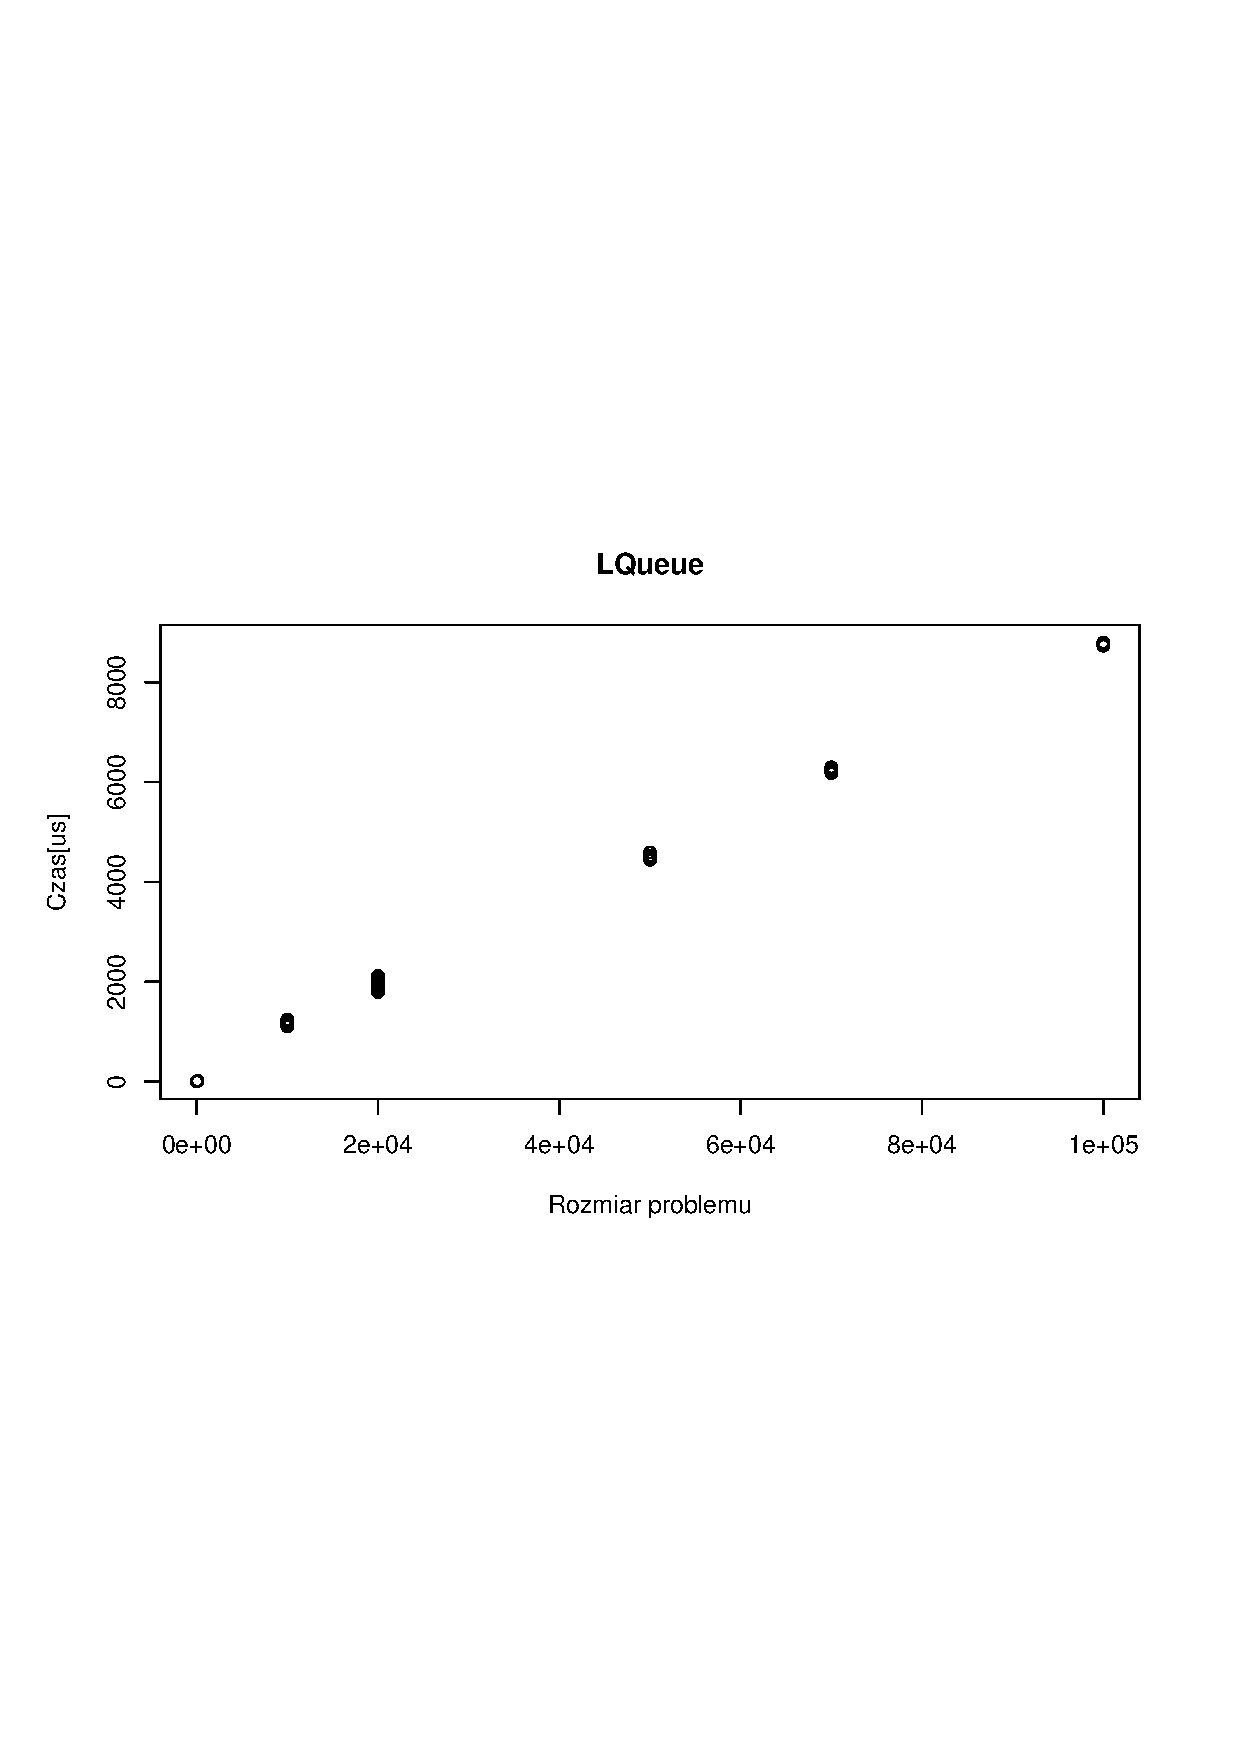
\includegraphics[width=0.7\linewidth]{./Wykresy/LQueue}
\caption{Kolejka zaimplementowana na liście}
\label{fig:LQueue}
\end{figure}

\begin{figure}[H]
\centering
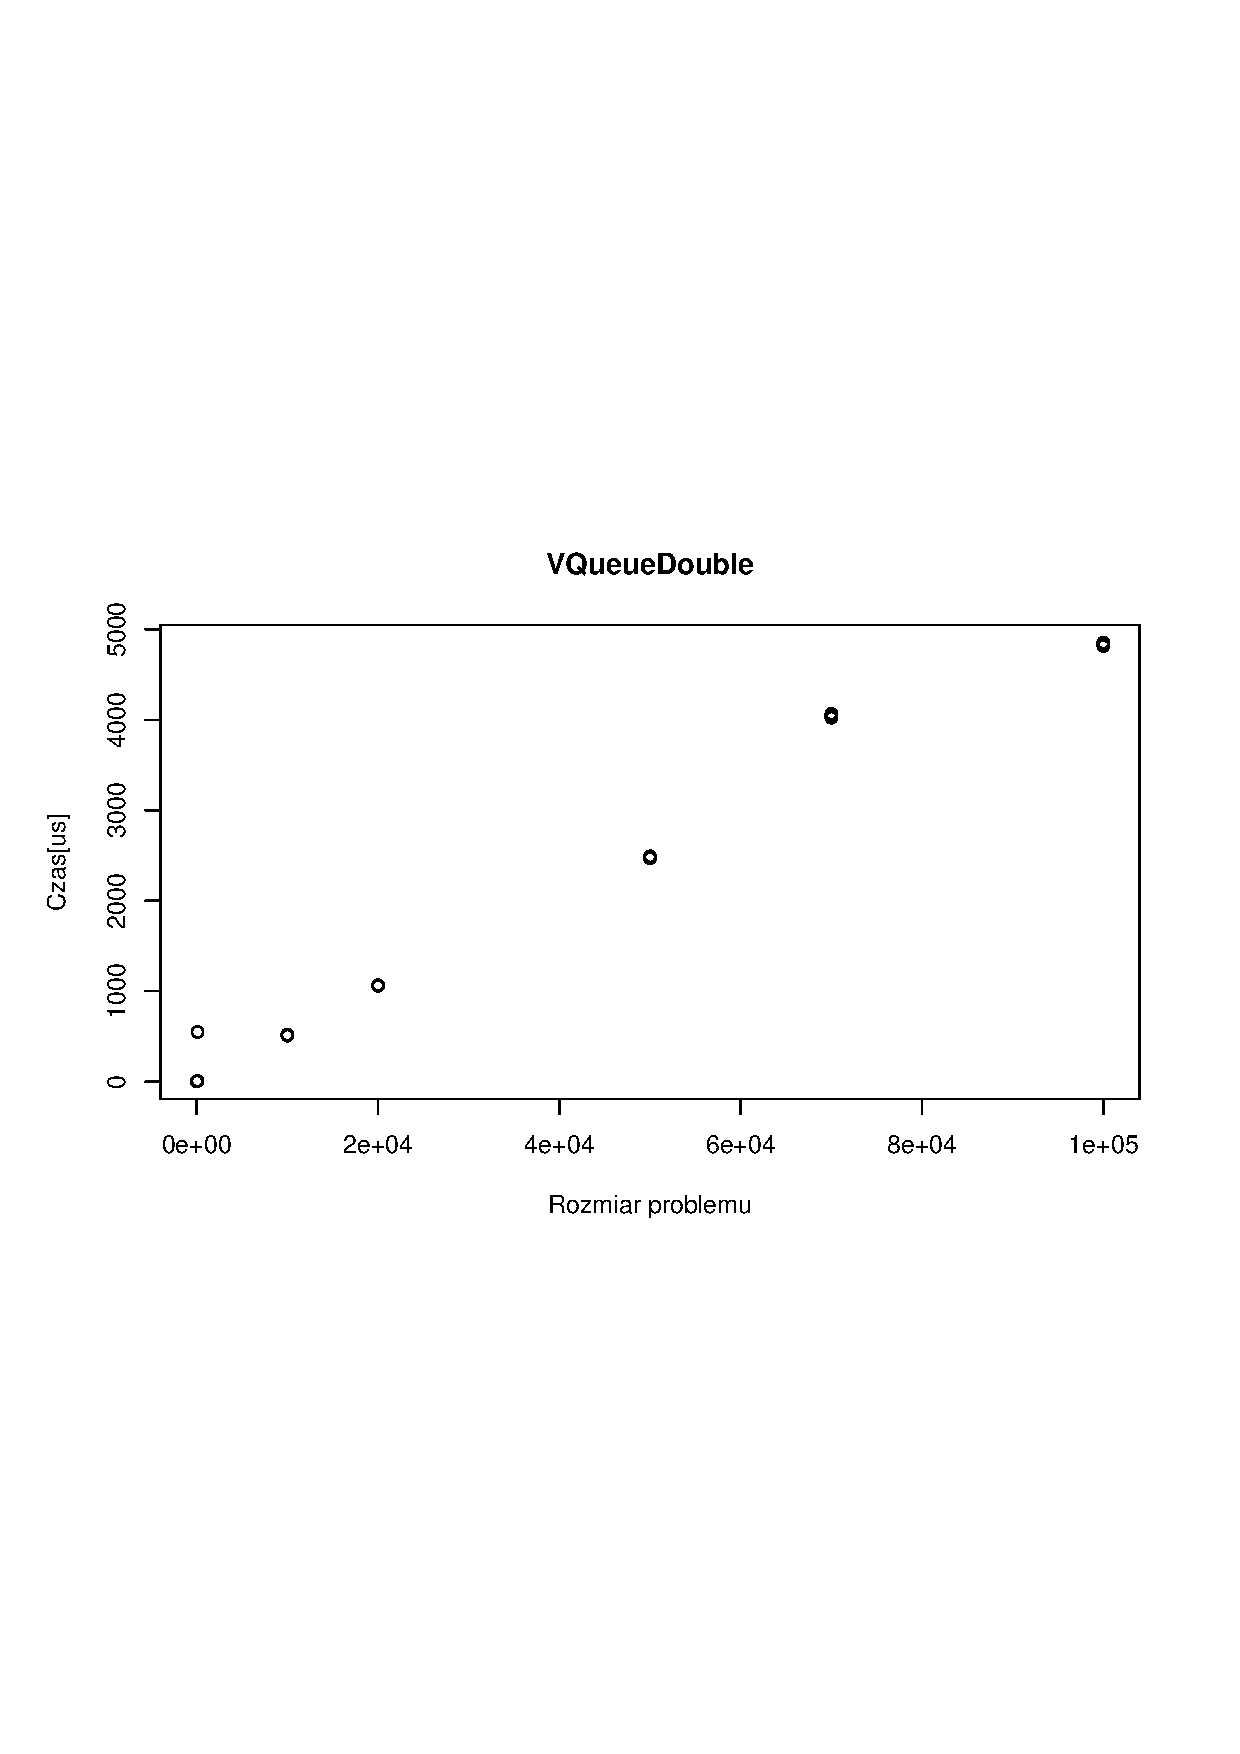
\includegraphics[width=0.7\linewidth]{./Wykresy/VQueueDouble}
\caption{Kolejka zaimplementowana na tablicy, metoda podwajania}
\label{fig:VQueueDouble}
\end{figure}

\begin{figure}
\centering
\includegraphics[width=0.7\linewidth]{./Wykresy/VQueueInc}
\caption{Kolejka zaimplementowana na tablicy, metoda inkrementacji}
\label{fig:VQueueInc}
\end{figure}


\subsection{Stos}

Przetestowałem stosy zaimplementowane na podstawie listy oraz tablicy. W przypadku tablicy
przetestowałem dwie różne metody alokacji pamięci, o których wspomniałem wcześniej. Wyniki 
prezentują się następująco:

\begin{figure}[H]
	\centering
	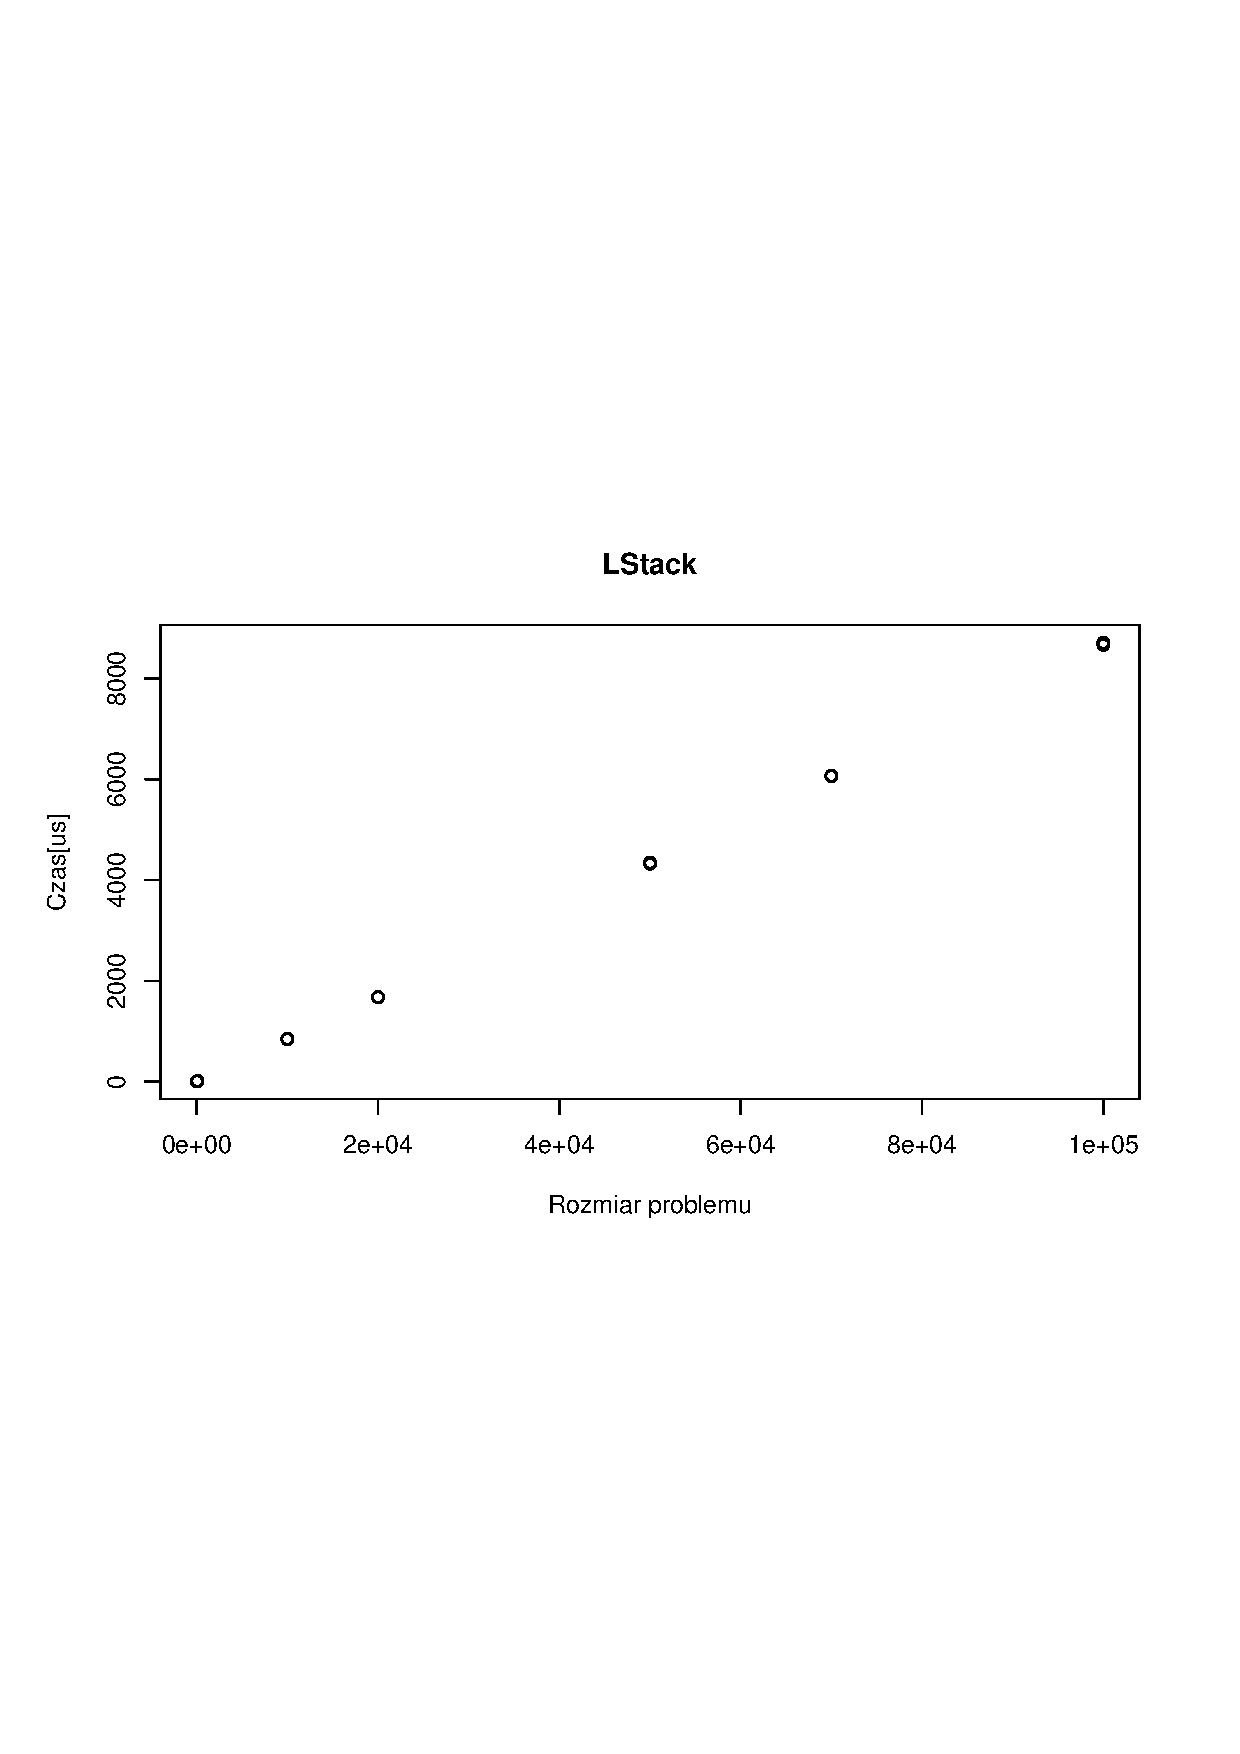
\includegraphics[width=0.7\linewidth]{./Wykresy/LStack}
	\caption{Stos zaimplementowany na liście}
	\label{fig:LStack}
\end{figure}

\begin{figure}[H]
	\centering
	\includegraphics[width=0.7\linewidth]{./Wykresy/VStackDouble}
	\caption{Stos zaimplementowany na tablicy, metoda podwajania}
	\label{fig:VStackDouble}
\end{figure}

\begin{figure}[H]
	\centering
	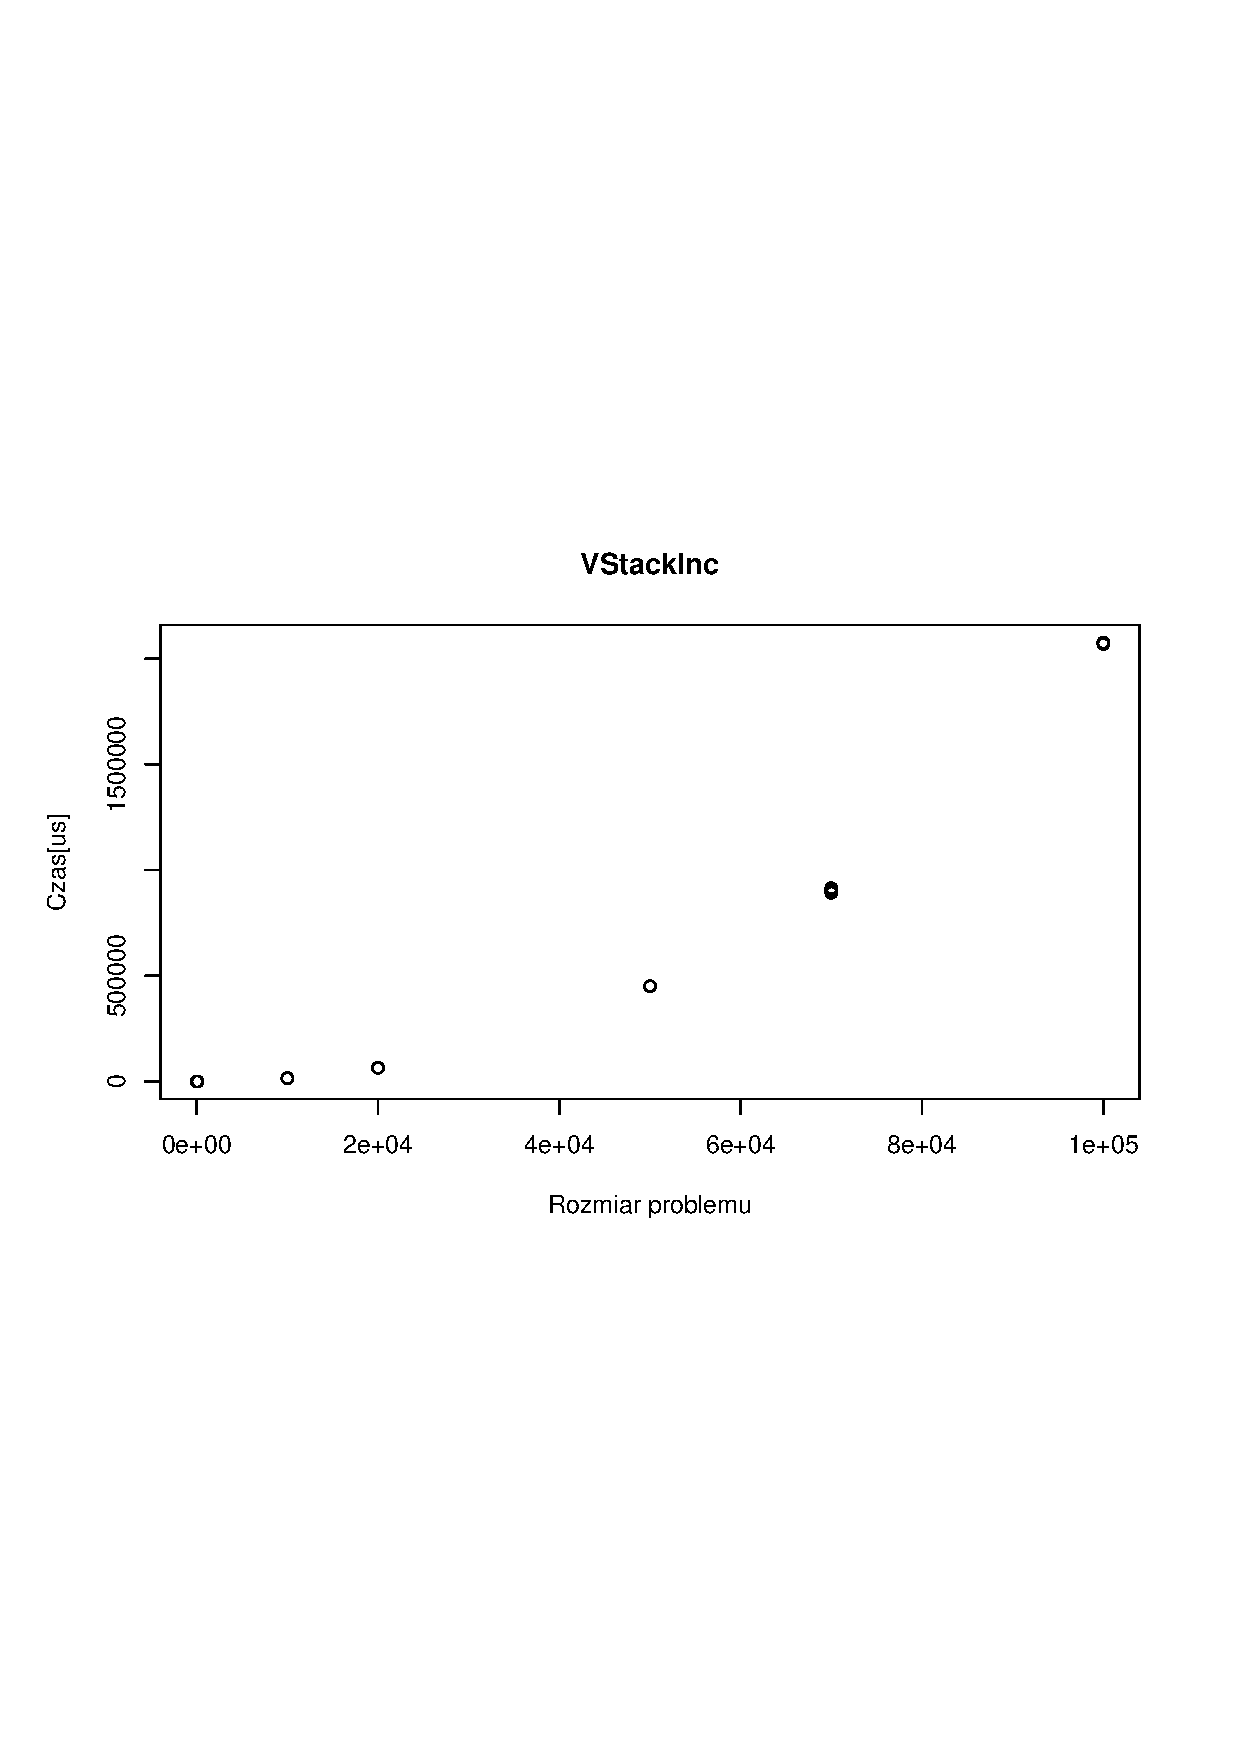
\includegraphics[width=0.7\linewidth]{./Wykresy/VStackInc}
	\caption{Stos zaimplementowany na tablicy, metoda inkrementacji}
	\label{fig:VStackInc}
\end{figure}

\section{Wnioski}
Na podstawie przeprowadzonych testów możemy wyciągnąć następujące wnioski:
\begin{itemize}
	\item Najgorszą implementacją jest implementacja na tablicy z alokacją inkrementacyjną
	\item Widać, że wrzucenie $n$ elementów na stos/kolejkę przy alokacji inkrementacyjnej
	 wiąże się ze złożonością $\mathcal{O}(n^2)$
	\item Przy implementacji za pomocą listy widać, że jest to złożoność liniowa
	\item Alokacja, w której podwaja się dostępny rozmiar w przybliżeniu jest liniowa,
	chociaż można dostrzec zbiory punktów, które do tej prostej nie należą - dla takiego rozmiaru
	przekopiowane musiały zostać dodatkowo wszystkie elementy
\end{itemize}

\end{document}